\documentclass[tikz,border=8pt]{standalone}
% Shared look for every TikZ diagram. Load with \input{../../tools/tikz-style.tex}
\usepackage[T1]{fontenc}
\usepackage{lmodern}
\renewcommand{\sfdefault}{lmr}  % diagrams use the same serif as the text
\usetikzlibrary{arrows.meta, positioning, shapes.geometric, calc, fit, backgrounds}
\definecolor{cblue}{HTML}{4C78A8}
\definecolor{corange}{HTML}{F58518}
\definecolor{cgreen}{HTML}{54A24B}
\definecolor{cred}{HTML}{E45756}
\definecolor{cpurple}{HTML}{B279A2}
\definecolor{cgrey}{HTML}{6B6B6B}
\tikzset{
  every picture/.style={font=\sffamily, line width=1.2pt},
  box/.style={draw=#1, fill=#1!12, rounded corners=4pt, align=center, inner sep=7pt, minimum height=1.1cm},
  box/.default=cgrey,
  arrow/.style={-{Stealth[length=3mm]}, draw=cgrey, line width=1.4pt},
  title/.style={font=\sffamily\bfseries\Large},
  note/.style={font=\sffamily\small, text=cgrey, align=center},
}
\AtBeginDocument{\hyphenpenalty=10000 \exhyphenpenalty=10000}

% Why the trailer turns. The hitch moves with the car: speed v along the car heading (40 deg). Relative to the
% trailer (heading 10 deg) that velocity splits into an along part v cos(30 deg) = 0.866 and an across part
% v sin(30 deg) = 0.5 (v = 1 m/s). The trailer's wheels cannot slide sideways, so the across part swings the
% trailer about its axle: turn rate = across speed / d_1 = 0.5 / 2 = 0.25 rad/s.
\begin{document}
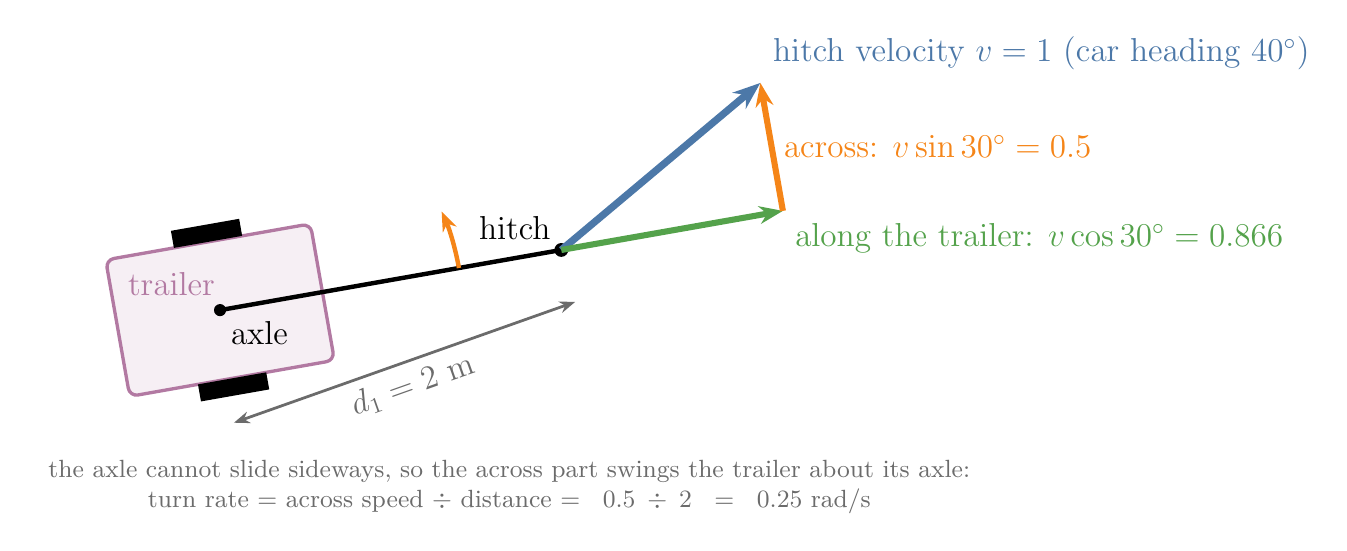
\begin{tikzpicture}[scale=2.2, every node/.append style={font=\large}]
  \coordinate (H) at (0,0);
  \coordinate (T) at ({-2*cos(10)},{-2*sin(10)});
  \begin{scope}[shift={(T)}, rotate=10]
    \draw[cpurple, fill=cpurple!12, rounded corners=3pt] (-0.6,-0.4) rectangle (0.6,0.4);
    \fill[black] (-0.2,0.4) rectangle (0.2,0.5); \fill[black] (-0.2,-0.5) rectangle (0.2,-0.4);
    \node[cpurple] at (-0.25,0.2) {trailer};
  \end{scope}
  \draw[black, line width=1.6pt] (T) -- (H);
  \fill[black] (H) circle (0.04); \fill[black] (T) circle (0.035);
  \node[below right] at (T) {axle};
  \node[above left] at (H) {hitch};
  % hitch velocity along the car heading
  \draw[-{Stealth[length=3.5mm]}, cblue, line width=2.6pt] (H) -- ({1.5*cos(40)},{1.5*sin(40)}) node[above right] {hitch velocity $v = 1$ (car heading $40^\circ$)};
  % split relative to the trailer axis (10 deg): along = 0.866, across = 0.5 (drawn x1.5)
  \draw[-{Stealth[length=3mm]}, cgreen, line width=2.2pt] (H) -- ({1.5*0.866*cos(10)},{1.5*0.866*sin(10)}) node[below right] {along the trailer: $v\cos 30^\circ = 0.866$};
  \draw[-{Stealth[length=3mm]}, corange, line width=2.2pt] ({1.5*0.866*cos(10)},{1.5*0.866*sin(10)}) -- ++({-1.5*0.5*sin(10)},{1.5*0.5*cos(10)}) node[midway, right] {across: $v\sin 30^\circ = 0.5$};
  % turning of the trailer about its axle
  \draw[-{Stealth[length=2.5mm]}, corange, line width=1.6pt] ($(T)+({1.4*cos(10)},{1.4*sin(10)})$) arc (10:24:1.4);
  \draw[{Stealth[length=2mm]}-{Stealth[length=2mm]}, cgrey, line width=1pt] ($(T)+(0.08,-0.65)$) -- ($(H)+(0.08,-0.3)$) node[midway, below, sloped] {$d_1 = 2$ m};
  \node[note, anchor=north, text width=12cm] at (-0.3,-1.15) {the axle cannot slide sideways, so the across part swings the trailer about its axle:\\turn rate $=$ across speed $\div$ distance $= 0.5 \div 2 = 0.25$ rad/s};
\end{tikzpicture}
\end{document}
